\documentclass{report}

% set font encoding for PDFLaTeX, XeLaTeX, or LuaTeX
\usepackage{ifxetex,ifluatex}

\if\ifxetex T\else\ifluatex T\else F\fi\fi T%
  \usepackage{fontspec}
\else
  \usepackage[T1]{fontenc}
  \usepackage[utf8]{inputenc}
  \usepackage{lmodern}
\fi

\usepackage{amsmath}
\usepackage{amssymb}
\usepackage{amsthm}
\usepackage{bm}
\usepackage{bbm}
\usepackage{mathtools}
\usepackage{physics}

\usepackage{enumitem}
\usepackage{multicol}
\usepackage{graphicx}
\usepackage[dvipsnames]{xcolor}

\usepackage{hyperref}
\hypersetup{colorlinks=true,}

\usepackage[parfill]{parskip}
\usepackage{lipsum}
\usepackage[export]{adjustbox}
\usepackage{listings}

\usepackage{xparse} 
\usepackage{subfig} 
\usepackage{xparse} 
\usepackage{float}

\usepackage[sorting=none]{biblatex} 

%%%%%This is an image table command, can likely be deleted
\newcommand{\subf}[2]{

%
{\small 
\begin{tabular}
  [t]{@{}c@{}} #1\ 
  \#2 
\end{tabular}
}

%
} 

\makeatletter
\renewcommand*\env@matrix[1][c]{\hskip -\arraycolsep
  \let\@ifnextchar\new@ifnextchar
  \array{*\c@MaxMatrixCols #1}}
\makeatother
%%%%%% Tensor Product
\NewDocumentCommand{\tens}{e{_^}}{ 
\mathbin{\mathop{\otimes}\displaylimits \IfValueT{#1}{_{#1}} \IfValueT{#2}{^{#2}} }}
%%%%%% Add \R Reals
\newcommand{\R}{\mathbb{R}} 
\newcommand{\N}{\mathbb{N}} 
\newcommand{\Z}{\mathbb{Z}} 
%%%%%% Missing citation warn
\newcommand{\CITEMISSING}{\colorbox{BurntOrange}{CITE ME}}
%%%%%% Add \theorem float
\newtheorem{theorem}{Theorem}
%%%%%% Add \definition float
\theoremstyle{definition} 
\newtheorem{definition}{Definition}[section]
%%%%%%%%%%%%%%%%%%%%%%%%%%%%%%%%%%%%%%%%%%%%%%%%%%%%%%%%%%%%%%%%%%%%%%%%%%%%%%%%%%%%%%%%%%%%%%%%%%%%%%%%%%%%%%%%%%%%%%%%%%
%%%%%Uncomment to add citation library 
\bibliography{lib}
\title{Model Description}
\author{David Helekal}

\begin{document}
\chapter{Model}
\section{Coalescent with Local Population Structure}
We now present novel local phylodynamic model.
In order to help illustrate the concepts behind this model, consider the following scenario:
Suppose there is a parent population of bacteria of interest evolving through time. At any point in time, a particular individual within this population gains a significant evolutionary advantage. This advantage enables the individual and its progeny to undergo a rapid clonal expansion as it gains the ability to colonise a particular niche, eventually reaching a constant population size equilibrium. We will associate the clade corresponding to the clonal expansion with a particular colouring. 
The clonal expansion process may repeat throughout time, giving rise to several clades. The clonal expansions may for example correspond to process such a bacterial strain gaining antibiotic resistance, or being newly introduced into a hospital.

In general, we will assume that the clonal expansion process happens relatively rarely. We will also assume the parent population is at eqillibrium. As under this scenario populations reach a constant population size in the limit this assumption can be interpreted that the clonal expansion that gave rise to the parent population has happened a very long time ago.

At present a researcher collects a random set of $N$ samples from the population of interest, containing at least some of the clades produced by the clonal expansion process described above. Each sample belongs to one of the $k$ clonal expansion clades with multinomial probability $\theta_i$, $\pmb{\theta} = [\theta_1, ..., \theta_i, ..., \theta_{k-1}, \theta_{k}]$.

The researcher then sequences the genomes of the samples and infers the corresponding phylogenetic using any of the popular available methods.
The resulting phylogeny can be viewed as a realisation of the following backwards time process. 

Select $K$ clade colours, and an associated clade sampling membership probability vector $\pmb{\theta}$. For each of the $N$ samples $s_i$ forming the leaves of the phylogeny, assign a colouring $c_i$. The samples of identical colour then coalesce with each other with rate governed by a colour specific population size function $\alpha_i(t)$. As it is assumed each colour is formed by a clonal expansion at time $t^{Div}_{i}$, $\alpha_i(t)$ vanishes to zero at the time of the expansion, and as such all coalescence within clade of colour $c_i$ happens almost surely before $t^{Div}_{i}$. Upon reaching the time of clonal expansion the MRCA then chnages colour to that of another clade extant at the time. The clade of the colour the MRCA changes to will be referred to as the parent clade. The MRCA is then added to the parent clade as a leaf. 
The process continues until all only one individual remains.

The coalescent process given leaf colouring and growth function parameters described above is characterised mathematically in the following section.
%%%%%%%%%%%%%%%%%%%%%%%%%%%%%%%%%%%%%%%%%%%%%%%%%%%%%%%%%%%%
%%%%%%%%%%%%%%%%%%%%%%%%%%%%%%%%%%%%%%%%%%%%%%%%%%%%%%%%%%%%
%%%%%%%%%%%%%%%%%%%%%%%%%%%%%%%%%%%%%%%%%%%%%%%%%%%%%%%%%%%%
%%%%%%%%%%%%%%%%%%%%%%%%%%%%%%%%%%%%%%%%%%%%%%%%%%%%%%%%%%%%
\subsection{Model}
\section{Preliminaries}
A given genealogy $\mathbf{g}=(V_\mathbf{g}, E_\mathbf{g}, t_\mathbf{g}, c_\mathbf{g})$ is an incomplete, empirical sample of the underlying process.\\
It consists of nodes $V_\mathbf{g}$, directed edges $E_\mathbf{g}$, node labels $t_\mathbf{g}$ corresponding to event times, and node labels $c_\mathbf{g}$ corresponding to node colouring.\\
The genealogy $\mathbf{g}$ shall be indexed by an index set $S=1\leq i \leq N\subset \N$, with $Y\subset S$ corresponding to coalescent events and $I\subset S$ corresponding to sampling events.\\
For convenience, assume that all edges are in the forwards time direction, i.e.: 
\begin{gather*}
\forall k,l \in S: (k,l)\in E_\mathbf{g} \Rightarrow t_k<t_l
\end{gather*}
Furthermore, all event times are ordered in descending (backwards) time order, with the first event corresponding the the most recent sample
\begin{gather*}
\forall k,l \in S: k<l \Rightarrow t_k > t_l
\end{gather*}
Under the assumption that $\mathbf{g}$ is a genealogy of a given sample, with each edge in $E_\mathbf{g}$ there is an associated unobserved set of individuals descending from one another. At some point along an edge from one lineage to another, the lineage can undergo a colour change, and become the most recent ancestor of a diverging clade. This event corresponds to this lineage somehow gaining advantage over other lineages, be it a bacterium gaining resistance against a drug, or a strain of a virus invading a completely susceptible population.

\begin{definition}[Multiple Lineage Coalescent]\label{def:model}
Given $M$ colours, $M$ population size functions $\mathbf{\alpha}\triangleq\{\alpha_j(t)\}_{1\leq j\leq M}$, the set of $M-1$ divergence times $T_{div} = \{t_{div_j}\}_{1\leq j<M}$, the set of $M-1$ divergence events $D = \{d_j\}_{1\leq j<M}$, the set of tips $I\subset \N, \quad I=\{1,2,...,N\}$, and the associated sampling times $T_{sam}\triangleq \left\{t^s_i\right\}_{i \in I}$.
Assume that the indexing is such that the divergence times are in ascending order.\\
Let $\pmb\Pi(t)$ be a continuous time markov chain defined on the state space of the partitions of $I$ denoted by $\Pi$, each associated with a colouring via the function $H: \Pi\cross\R^+ \mapsto \{1,...M\}$. The initial state is given by $\pmb\Pi(0) = \{1\}, \{2\}, ... , \{N-1\}, \{N\}$.

Denote the number of extant partitions of given colour $j$ at time $t$ by $|C_j(t)| \triangleq |\{\pi \in \Pi(t) : H(\pi, t) = j \}|$

And transition rates
\begin{gather}\label{eq:transitions}
q_{(\pi_i,\pi_j), (\pi_i\cup\pi_j)}=\lim\limits_{h \downarrow 0}\frac{1}{h}\mathbf{P}\left[\pi_i \cup \pi_j \in \pmb\Pi(t+h)\mid \pi_i, \pi_j \in \pmb\Pi(t), \pi_i \neq \pi_j \right]  
\end{gather}
given by
\begin{gather}\label{eq:rates}
q_{(\pi_i,\pi_j), (\pi_i\cup\pi_j)} = \sum\limits_{k=1}^{M} \delta_k(H(\pi_i,t))\delta_k(H(\pi_j,t))\frac{\binom{C_k(t)}{2}}{\alpha_k(t)}
\end{gather}
\end{definition}
Finally, $H$ is defined recursively with $\forall \pi_i \in \pmb\Pi(0), H(\pi_i,0) = c_{i,0}$ with $c_{i,0}$ given. For fixed $t$ and and $\forall \pi \in \pmb\Pi(t)$, The colouring function satisfies $H(\pi, t) = H(\pi_0,t)\quad \forall \pi_0 \in \pmb\Pi(0) : \pi_0 \subset \pi$. In time, $H$ is defined so that $\forall \pi \in \pmb\Pi(0) : H(\pi,0) = j,\quad \forall t>0 \quad H(\pi, t) = \begin{cases} 
      j & t < T_{div_j} \\
      d_j & t \geq T_{div_j}
   \end{cases}$\\
   
While the model is defined in terms of partitions, when working with genealogies we typically work with trees. The tree corresponding to a particular realisation of the partition based model is obtained by identifying all $\pi \in \pmb\Pi(t)\forall t$ with $V_\mathbf{g}$. The leaves $V_I$ consist of all partitions $\pi \in \pmb\pi(0)$, while internal nodes $V_Y$ consist of all subsequent partitions $\forall t, \forall\pi\in \pmb\Pi(t) : \pi \notin \pmb\Pi(0)$. The edges $V_\mathbf{g}$ and times $t_\mathbf{g}$ are given by the jump chain. The colouring $c_\mathbf{g}$ is obtained through the colouring function $H$. 

The interpretation of this model in backwards (coalescent) time is that each node corresponds to a single specific clade (colour). Nodes of the same clade coalesce at i.i.d rates, according to a clade specific growth functions, until reaching the most recent common ancestor (MRCA) of given clade. The MRCA then changes type (colour) to that given by the corresponding divergence event at corresponding divergence time time. 

Within-colour transitions and their rates are independent of different colours. As such the transitions involving partitions of one colour  are independent of transitions involving partitions of other colours given divergence events and times. This allows us to split the likelihood computation into a product of colour-specific likelihoods, that can be computed under coalescent with variable population size.\\

%%%%%%%%%%%%%%%%%%%%%%%%%%%%%%%%%%%%%%%%%%%%%%%%%%%%%%%%%%%%
%%%%%%%%%%%%%%%%%%%%%%%%%%%%%%%%%%%%%%%%%%%%%%%%%%%%%%%%%%%%
%%%%%%%%%%%%%%%%%%%%%%%%%%%%%%%%%%%%%%%%%%%%%%%%%%%%%%%%%%%%
%%%%%%%%%%%%%%%%%%%%%%%%%%%%%%%%%%%%%%%%%%%%%%%%%%%%%%%%%%%%
\section{Full Model}
Given a population sample of $N$ individuals indexed by $F$, $X_F = \{x_i\}_{i \in F}$, first determine the number of recent clonal expansions $M-1$:
\begin{gather}
M-1 \sim \texttt{poi}(\phi)
\end{gather}
Then simulate the $M$ clonal expansion probability vector $\pmb{\theta}$:
\begin{gather}
\pmb{\theta} \sim \texttt{dirichlet}(\psi), \quad \psi \in \R_+^{M} 
\end{gather}
Given the number of expansions $M-1$ and expansion probabilities $\pmb{\theta}$, partition $F$ into $M$ mutually disjoint subsets $\mathbf{f}=\{f_1, ... f_M-1, f_{M}\}$ with $\bigcup\limits_{i=1}^{M} f_{i} = F$ with the probability $P[j\in f_{i}]=\theta_i\quad \forall i,\forall j \in F$.  
Each partition corresponds to an individual colour characterising a clonal expansion. For convenience, we will set $f_{M}$ to be the index set of the tips corresponding to the parent subpopulation.

The sample along with the initial colour assignment then follows the coalescent process described above in \ref{def:model}, governed by population size functions $\alpha^{-1}_{j}(t)$. To each $\alpha^{-1}_{j}$ corresponds a set of parameters:
\begin{gather}
\begin{aligned}
t_{div_{j}}\in\R_+ \quad&\text{The time of divergence}\\
r_j\in\R_+\quad&\text{The growth rate of the subpopulation}\\
N_j\in\R_+\quad&\text{The carrying capacity}
\end{aligned}
\end{gather}
The divergence events $d_i$ are simulated so that an expansion with divergence time $t_{div_j}$ merges with and thus changes colour to that of an expansion chosen uniformly at random from all expansions with time of divergence after $t_{div_j}$, i.e. an expansion that is extant at time $t_{div_j}$.

In the case of the parent subpopulation $f_{M}$, we assume that the divergence event happened a very long time ago. As by definition $\alpha(t) \rightarrow N$ as $T_{div}-t\rightarrow -\infty$, we approximate $\alpha_{M}(t) \approx N_{M}$ and as such $\alpha^{-1}_{M}(t) \approx 1/N_{M}$. The parameters $T_{div_{j}}, r_j, N_j$ are simulated from appropriate (prior) distributions.
Finally, without loss of generality, assume that divergence events are indexed in ascending order by the time of divergence in coalescent time.
\begin{gather}
i > j \Leftrightarrow T_{div_i} > T_{div_j}  
\end{gather}
Sampling times $\mathbf{t}=\{t_i\}_{i\in F}$ are simulated from the same distribution for all $f$. It is required that for all expansions $j$, $t_i < T_{div_j}$, for all $i \in f_j$. In other words, all sampling for a given clade must happen after the clade diverges.
\subsubsection{Choice of effective population size functions}
While the parent clade is assumed to be at equilibrium, the population size functions of the diverging clades have to satisfy several properties.\\
First we introduce the variable $\tau = -t - T_{max} + T_{div}$ which denotes time relative to a divergence event of a given clade, where $T_{div}$ denotes the divergence time and $T_{max}$ denotes the time of the most recent sample.
In our model we assume that the diverging subpopulation only appears after the divergence event, and as such it is required that at time $\tau=0$ the population vanishes $\alpha(\tau)=0$. Furthermore, we are looking for a monotone decreasing function in $\tau$, that exhibits saturating behaviour as $\tau$ grows large.
Initially, functions exhibiting a period of exponential growth were investigated, however these were ill-posed numerically.
Hence we arrived at the following function
\begin{gather}
\alpha(\tau) = N\frac{r\tau^2}{1+r\tau^2}
\end{gather} 
Where $N$ is the carrying capacity and $r$ is the growth rate.
This function  exhibits saturating behaviour, symmetry around zero, and numerically stable behaviour.\\
While the intepretation of the carrying capacity $N$ is straightforward, we find $r$ to be best intepreted by considering the time to when the population reaches half the carrying capacity $T_mid$ as a function of $r$. It is straightforward to show that $T_{mid}(r) = \frac{1}{\sqrt{r}}$ 
\begin{figure}[H].
  \centering
     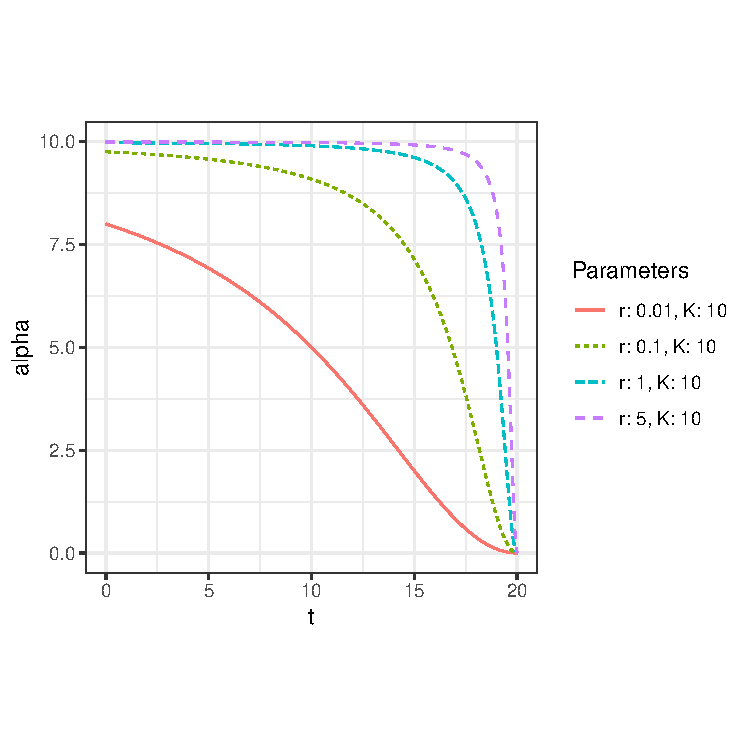
\includegraphics[width=0.4\textwidth]{../R/test_mcmc/alpha_plots}
    \caption{$\alpha(\tau)$ under different parameters, with $T_{div}=20$}
\end{figure}
The integral of the reciprocal $\alpha^{-1}(\tau)$ under this formulation is then given by 
\begin{gather}
\begin{aligned}\label{eq:rint}
&\int_{t}^{t+s}\alpha^{-1}(\tau)\,d\tau\\ &= \frac{1}{N}\left[-\frac{1}{r(-\tau-T_{max}+T_{div})}-\tau-T_{max}+T_{div}\right]_{t}^{t+s}
\end{aligned}
\end{gather}
As $t+s$ approaches the divergence time relative to the most recent sample $T_{div} - T_{max}$, the rate integral \ref{eq:rint} approaches infinity, and as such all coalescence within a clade happens before time of divergence with probability one.

For the purposes of our model, we simulate the parameters $N_j, r_j, t_{div_j} \forall j \in \{1,...,M-1\}$ as well as the parent population size $N_{M}$ under the following scheme.\\
First simulate the parent population size $N_{M}$:
\begin{gather}
N_{M} \sim \texttt{lognorm}(\mu_{anc}, \sigma_{anc})
\end{gather}
Next simulate the carrying capacities for the $M-1$ expansions
\begin{gather}
N_{j} \sim \texttt{lognorm}(N_{M}, \sigma_{exp}) \quad\forall j \in \{1,...,M-1\}
\end{gather}
as well as the corresponding divergence times
\begin{gather}
t_{div_j} \sim U\{(\beta N_{M}, N_{M})\} \quad\forall j \in \{1,...,M-1\}
\end{gather}
where $\beta \in (0,1)$
and growth rates
\begin{gather}
r_{j} \sim \texttt{lognorm}(\mu_r, \sigma_r) \quad\forall j \in \{1,...,M-1\}
\end{gather} 
\subsubsection{Summary}
We now summarise the entire simulation procedure
\begin{gather}
\begin{aligned}
&\pi(M-1) &=& \texttt{poi}(\phi) &\quad&\text{Number of expansions} \\
&\pi(\pmb\theta\mid M) &=& \texttt{dirichlet}(\psi) &\quad&\text{Expansion Membership Probabilities} \\
&\pi(\mathbf{f\mid\pmb\theta}) &=& \texttt{multinom}(\theta; M) &\quad&\text{Expansion Membership Assignment} \\
&\pi(N_M) &=& \texttt{lognorm}(\mu_{anc},\sigma_{anc}) &\quad&\text{Parent Population Size}\\
&\pi(N_j\mid N_{M}) &=& \texttt{lognorm}(N_{M},\sigma_{exp}) &\quad&\text{Carrying Capacities}\\
&\pi(t_{div_j}\mid N_{M}) &=& U\{(\beta N_{M},N_{M})\} &\quad&\text{Expansion Times}\\
&\pi(r_j) &=& \texttt{lognorm}(\mu_{r},\sigma_{r}) &\quad&\text{Growth Rates}\\
&\pi(d_j) &=& U\{\{i\in \{1 ... M+1\} : i > j\}\} &\quad&\text{Parent Populations}\\
\end{aligned}
\end{gather}

For convenience, we will summarise $\pi(N_M)\pi(N_j\mid N_{M})\pi(t_{div_j}\mid N_{M})\pi(r_j) \quad \forall j$ as $\pi(\pmb\alpha)$ and $\pi(t_{div_j}\mid N_{M})\quad \forall j$ as $\pi(T_{div}\mid\pmb\alpha)$

The tip times $T_{sam}$ are simulated separately and considered given. Furthermore $T_{sam} \perp M, \mathbf{f}, \pmb{\theta}, \pmb\alpha, D, T_{div}$.

The genealogy $\mathbf{g}$ is simulated under the Coalescent with Local Population structure described in \ref{def:model} denoted by $\texttt{lpcoal}$:
\begin{gather}
\pi(\mathbf{g}\mid M, \mathbf{f}, \pmb\alpha, T_{div}, D, T_{sam}) = \texttt{lpcoal}(M, \mathbf{f}, \pmb\alpha, T_{div}, D, T_{sam})
\end{gather} 

$\phi, \psi, \mu_{anc}, \sigma_{anc}, \mu_r, \sigma_r, \sigma_{exp}, \beta$ are hyperamaters and considered given.


%%%%%%%%%%%%%%%%%%%%%%%%%%%%%%%%%%%%%%%%%%%%%%%%%%%%%%%%%%%%
%%%%%%%%%%%%%%%%%%%%%%%%%%%%%%%%%%%%%%%%%%%%%%%%%%%%%%%%%%%%
%%%%%%%%%%%%%%%%%%%%%%%%%%%%%%%%%%%%%%%%%%%%%%%%%%%%%%%%%%%%
%%%%%%%%%%%%%%%%%%%%%%%%%%%%%%%%%%%%%%%%%%%%%%%%%%%%%%%%%%%%
\subsection{Posterior}
The posterior for the full process is:
\begin{gather}
\begin{aligned}
P(k, \mathbf{f}, \pmb{\theta}, \pmb{T_{div}}, \mathbf{r}, \mathbf{N}\mid\mathbf{g})
&\propto \pi(\mathbf{g}\mid M, \mathbf{f}, \pmb\alpha, T_{div}, D)\\
&\cross \pi(\pmb\alpha\mid M)\\
&\cross \pi(D\mid M)\\
&\cross \pi(\mathbf{f}\mid\pmb{\theta}, M)\\
&\cross\pi(\pmb{\theta}\mid M)\pi(M)
\end{aligned}
\end{gather}

\chapter{References}
\printbibliography
\end{document}